\subsection{连分式法}
\begin{frame}{连分式法}
     终点$p$的信息椭圆在只有锚点定位的情况下是一个圆。

%  \begin{columns}[T] % contents are top vertically aligned
 %    \begin{column}[T]{7cm}
     \begin{equation*}
    T_1=\lambda
     \end{equation*}
  %    \end{column}
   %  \begin{column}[T]{3cm} % alternative top-align that's better for graphics
        \begin{figure}
          \centering
          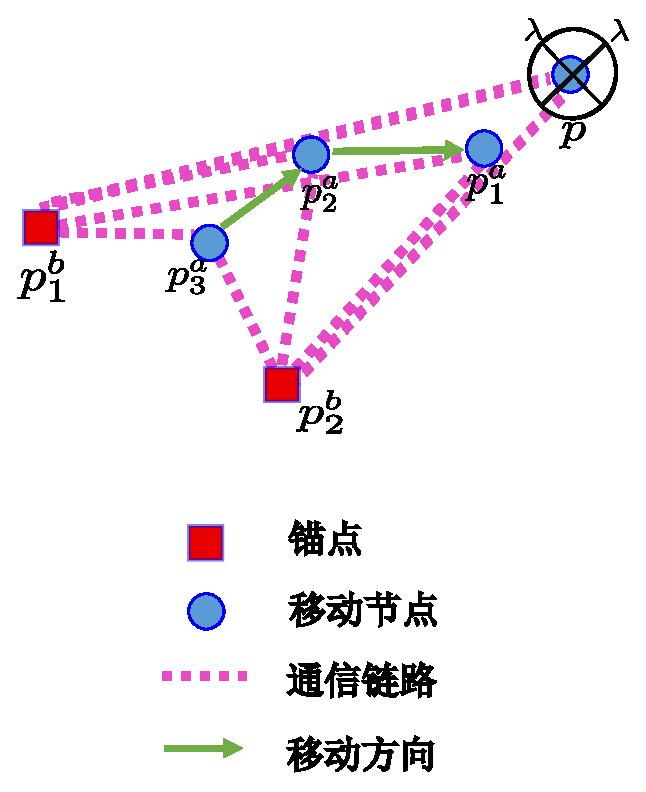
\includegraphics[width=120pt]{direct_single_temporal_pre.eps}
        \end{figure}
    % \end{column}
    % \end{columns}
  \end{frame}
  \begin{frame}
     增加了和上一时刻的协作链路后终点$p$的信息椭圆在沿$\bm{p}\bm{p}_1^a$方向上的信息$T_1$可以写成连分式的形式:
     \begin{equation*}
T_1=\lambda+\cfrac{1}{1+\cfrac{\sin^2 \theta_1}{\lambda}+\cfrac{\cos^2\theta_1}{\lambda+\cfrac{1}{1+\cfrac{\sin^2 \theta_2}{\lambda}+\cfrac{\cos^2\theta_2}{\lambda+\boxed{\cfrac{1}{1+\cfrac{1}{\lambda}}}}}}}.
     \end{equation*}
%\raggedright{
%\fbox{\includegraphics[width=160pt]{../presentation/direct_single_normal.eps}}
%}
%\vskip -9em
%\parbox[c][6em][t]{0.33\textwidth}{距$\bm{p}$较远的节点$\bm{p}_3^a$提供的信息在连分式的最内侧}
\begin{tabular}{lr}
\multirow[t]{4}{*}[-3em]{\fbox{\includegraphics[width=160pt]{direct_single_normal.eps}}}&\parbox[c][6em][t]{0.33\textwidth}{距$\bm{p}$较远的节点$\bm{p}_3^a$提供的信息在连分式的最内侧}\\
\end{tabular}
%\fbox{\includegraphics[width=160pt]{../presentation/direct_single_normal.eps}}
  \end{frame}

    \begin{frame}
     考虑增加一个角度参数$\theta_{N_a}$,由此得到的新的$T_1$记为$T'_1(N_a)$,研究$T'_1(N_a)$比原来的$T_1(N_a)$增大的量。
%  \begin{columns}[T] % contents are top vertically aligned
 %    \begin{column}[T]{7cm}
 \begin{equation*}
T'_1=\lambda+\cfrac{1}{1+\cfrac{\sin^2 \theta_1}{\lambda}+\cfrac{\cos^2\theta_1}{\dots+\cfrac{\dots}{1+\cfrac{\sin^2 \theta_3}{\lambda}+\cfrac{\cos^2\theta_3}{\lambda+\cfrac{1}{1+\cfrac{1}{\lambda}}}
}}}.
     \end{equation*}
%     \vskip -6em
  %   \end{column}
   %  \begin{column}[T]{3cm} % alternative top-align that's better for graphics
 \raggedright{
\fbox{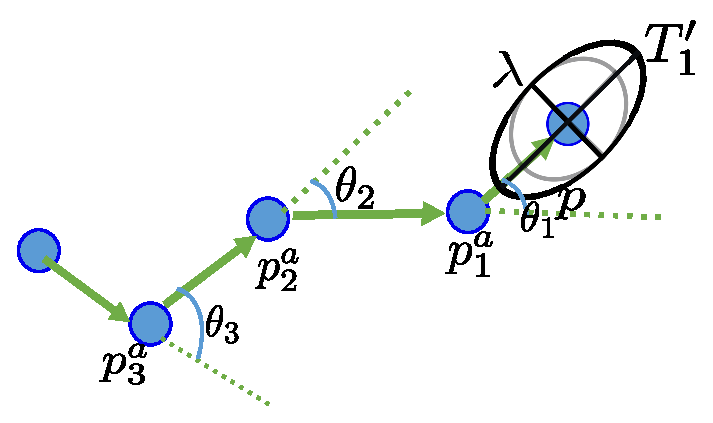
\includegraphics[width=160pt]{direct_single_normal_after.eps}}
}
%\vskip -6em

%         \quad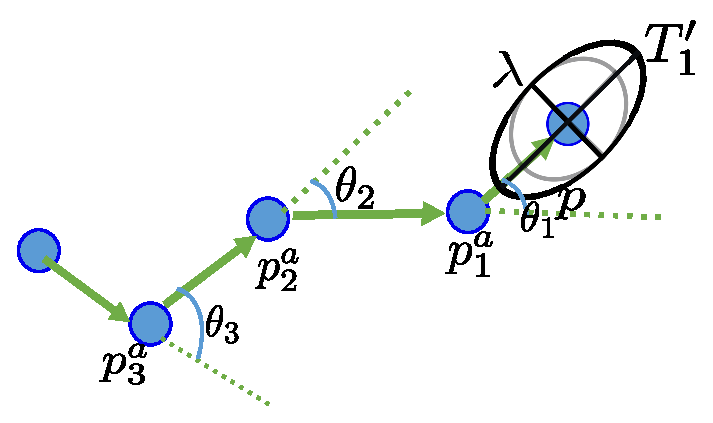
\includegraphics[width=120pt]{direct_single_normal_after.eps}
    % \end{column}
     %\end{columns}
  \end{frame}
\begin{frame}
一般地,可以得到终点时刻信息椭圆短轴方向的特征值为$\lambda$,长轴方向的特征值$T_1$可以用连分式表示。

设$\bm{u}_i=(\cos\theta_i,\sin\theta_i)^{\textrm{T}}$
\begin{equation*}
\begin{split}
T_{i-1} =& \lambda + \frac{1}{1+\frac{\sin^2\theta_i}{\lambda}+\frac{\cos^2\theta_i}{T_i}},2\leq i\leq N_a-1\\
T_{N_a-1}  =& \lambda+\frac{1}{1+1/\lambda}
\end{split}
\end{equation*}

%$T_1$就是$U_{N_a}$的另一个特征值。
\pause
记增量$\Delta_+ T_1(N_a):=T'_1(N_a)-T_1(N_a)$,则我们可以得到
%$N_a=1$时有$\Delta_{+} T_{1}=\frac{\lambda}{\lambda+1}$,
$N_a\geq 2$时$\Delta_+ T_1(N_a)$满足:
\begin{equation*}
%\begin{split}
%\frac{(\cos\Delta\theta)^{2(N_a-1)}}{(1+1/\lambda)^2(\lambda^2+2\lambda)(2+\lambda)^{2(N_a-2)}}\leq & \Delta_+ T_1(N_a)\\
\Delta_+ T_1(N_a)\leq \frac{1}{(\lambda^2+2\lambda)(1+\lambda)^{2(N_a-2)}}.
%\end{split}
\end{equation*}
从而得到$N_a\to \infty$时$T_1$的收敛性。
%$T_1$是关于$\theta_1,\dots,\theta_{N_a-1}$的减函数,关于$N_a$的增函数。
\end{frame}
\begin{frame}
基于连分式法,取$\theta_i \sim U[0,2\pi]$的随机数,增量$T_1'(N_a)-T_1(N_a)$随$N_a$变化的仿真结果如下图所示
\begin{figure}
  \centering
  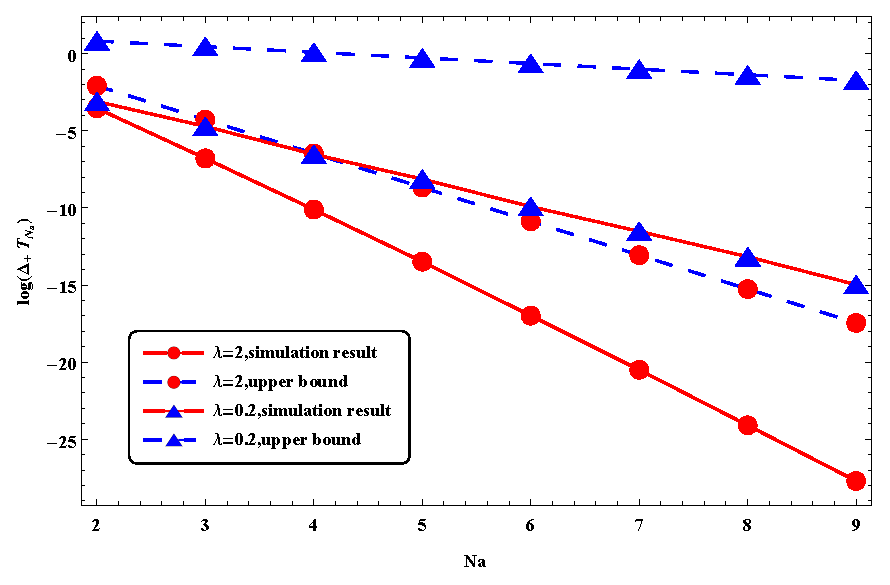
\includegraphics[width=280pt]{decreasing_exponential.eps}
  \caption*{协作链路信息衰减图示}\label{fig:continuous_fraction_exponential}
\end{figure}
\end{frame}
\begin{frame}
\begin{columns}[c]
 \begin{column}{.5\textwidth} % column designated by a command
 \begin{block}{衰减规律}
$N_a$条链路之外增加一层协作链路使目标节点定位误差的下降的数量是随$N_a$\alert{指数衰减}的。
\end{block}
\begin{block}{工程启示}
对某时刻的节点进行定位时,只需考虑其前后几个时刻的位置即可,较远的时刻基本没有信息量。
\end{block}
\end{column}
    \begin{column}{.5\textwidth}
       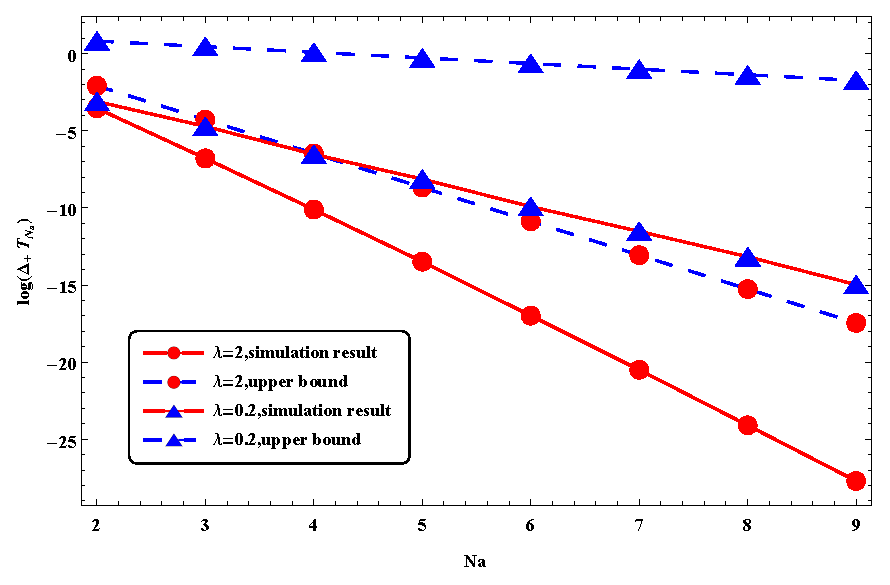
\includegraphics[width=160pt]{decreasing_exponential.eps}
       \end{column}
    \end{columns}
%为说明此结论,使用下面的记号
%\[
%[t_1,t_2,\dots,t_{n-1},t_n]=t_1+\cfrac{1}{t_2+\cfrac{1}{t_3+\dots+\cfrac{1}{t_{n-1}+\cfrac{1}{t_n}}}}
%\]
\end{frame}
%\begin{frame}{连分式的基本知识}
%\framesubtitle{有理数的有限连分式展开}
%\[
%\frac{682}{305}=2+\frac{72}{305}+2+\frac{1}{305/72}=2+\cfrac{1}{4+\cfrac{17}{72}}=\dots=2+\cfrac{1}{4+\cfrac{1}{4+\cfrac{1}{4+1/4}}}
%\]
%\end{frame}
%\begin{frame}
%\begin{itemize}
%  \item {欧几里得辗转相除法
%                \begin{eqnarray*}
%                 % \nonumber % Remove numbering (before each equation)
%                   682 =305\times2+72 & q_0=2\\
%                   305 = 72\times4+17 & q_1=4\\
%                   \dots = \dots& \\
%                   4 = 1\times4 &q_n=4
%                 \end{eqnarray*}
%                 }
%  \item {一个有理数表示为分数,一个分数看成两个整数的除法,可以用欧几里得法分解得出一系列的商$q_i$,
%  \[
%  \frac{682}{305}=q_0+\cfrac{1}{q_1+\cfrac{1}{q_2+\dots+1/q_n}}
%  \]
%  }
%\end{itemize}
%\end{frame}
%\begin{frame}{无理数的连分式展开}
%\begin{eqnarray*}
%\sqrt{5}=2+x_0&0<x_0<1\\
%\frac{1}{x_0}=4+x_1&0<x_1<1\\
%\dots&\dots\\
%\frac{1}{x_{n-1}}=4+x_n&0<x_n<1
%\end{eqnarray*}
%\[
%\sqrt{5}=2+\cfrac{1}{4+\cfrac{1}{4+\cfrac{1}{4+\dots}}}
%\]
%\end{frame}
%\begin{frame}
%记增量$\Delta_+ T_1(N_a):=T'_1(N_a)-T_1(N_a)$,则我们有如下结论:
%$N_a=1$时有$\Delta_{+} T_{1}=\frac{\lambda}{\lambda+1}$,
%
%$N_a\geq 2$时$\Delta_+ T_1(N_a)$满足:
%\begin{equation*}
%\begin{split}
%\frac{(\cos\Delta\theta)^{2(N_a-1)}}{(1+1/\lambda)^2(\lambda^2+2\lambda)(2+\lambda)^{2(N_a-2)}}\leq & \Delta_+ T_1(N_a)\\
%\Delta_+ T_1(N_a)\leq & \frac{1}{(\lambda^2+2\lambda)(1+\lambda)^{2(N_a-2)}}.
%\end{split}
%\end{equation*}
%\pause
%
%上式中
%\[
%\Delta \theta=\max_{2\leq k \leq N_a-1}|\theta_k|,\theta_k\leq \frac{\pi}{2}
%\]
%\end{frame}
\begin{frame}
$T_1$是关于$\theta_1,\dots,\theta_{N_a-1}$的减函数,关于$N_a$的增函数。

$T_1$方向上的信息量有一个上界,当诸夹角均趋于0且时间协作数量$N_a\to \infty$,这个上界可以达到:
\begin{equation*}
\lim_{\Delta \theta\to 0,N_a\to \infty}T_1(N_a)=\frac{\lambda+\sqrt{\lambda^2+4\lambda}}{2}
\end{equation*}
其中
\[
\Delta \theta=\max_{2\leq k \leq N_a-1}|\theta_k|
\]

%因为如果某个$\theta_i$等于90度,那么有限连分式$T_1$中就在$\theta_i$处截断了。
\end{frame}



%\begin{definition}
%  序列$t_1,t_2,\dots,t_r$;对于$j\geq2$可以递推地定义有限连分式$[t_1,t_2,\dots,t_r]:=t_1+\frac{1}{[t_2,\dots,t_r]}$
%\end{definition}
%比如
%\begin{align*}
%[2,4,4,4,4]&=2+\frac{1}{[4,4,4,4]}\\
%&=2+\frac{1}{4+\frac{1}{[4,4,4]}}
%\end{align*}
%一个有限连分式从定义上来说是从后往前算的,下面的定理指出可以从前往后算:
%\end{frame}
%\begin{frame}
%\begin{theorem}\label{thm:basic}
%设$a_{-1}=0,b_{-1}=1;a_0=1,b_0=0;$\\
%$a_n=t_n a_{n-1}+a_{n-2},b_n=t_n b_{n-1}+b_{n-2};n\geq 1$
%那么
%\begin{align*}
%[t_1,t_2,\dots,t_n]&=\frac{a_n}{b_n}\\
%&=\frac{t_n a_{n-1}+a_{n-2}}{t_n b_{n-1}+b_{n-2}}
%\end{align*}
%  设$p_j=t_j p_{j-1}+p_{j-2},q_j=t_j q_{j-1}+q_{j-2}$,$M_j=(\begin{matrix}p_j&q_j\\p_{j-1}&q_{j-1}\end{matrix})$
%  $p_0,p_1,q_0,q_1$由$M_0=I_2$给出,$T_j=(\begin{matrix}t_j&1\\1&0\end{matrix})$
%  则$M_j=T_jM_{j-1}$,递推得到$\binom{p_j}{q_j}=(\prod_{i=1}^r T_i )\binom{1}{0}$且
%  $[t_1,t_2,\dots,t_r]=\frac{p_r}{q_r}$
%\end{theorem}
%比如为计算$[2,4,4,4,4]\approx 2.236$
%\begin{tabular}{lll}
%  % after \\: \hline or \cline{col1-col2} \cline{col3-col4} ...
%  $a_1=2a_0+a_{-1}=2$ & $b_1=2b_0+b_{-1}=1$ &$[2]=\frac{a_1}{b_1}=2$ \\
%  $a_2=4a_1+a_0=9$ & $b_2=4b_1+b_0=4$ & $[2,4]=\frac{a_2}{b_2}=2.25$\\
%  $a_3=4a_2+a_1=38$ & $b_3=4b_2+b_1=17$ & $[2,4,4]=\frac{a_3}{b_3}=2.235$\\
%  \dots &\dots &\dots
%\end{tabular}
%\end{frame}
%\begin{frame}
%关于定理\ref{thm:basic}的理解:
%化简后是关于z的分式线性变换:
%\[
%[t_1,t_2,\dots,t_{n-1},z]=\frac{az+a'}{bz+b'}
%\]
%考虑$z\to \infty$得$[t_1,t_2,\dots,t_{n-1},z]\to[t_1,t_2,\dots,t_{n-1}]$
%\[
%\Longrightarrow \frac{a}{b}=\frac{a_{n-1}}{b_{n-1}}
%\]
%\end{frame}
%\begin{frame}
%\[
%[t_1,t_2,\dots,t_{n-1},z]=\frac{az+a'}{bz+b'}
%\]
%考虑$z\to 0$得$[t_1,t_2,\dots,t_{n-1},z]\to[t_1,t_2,\dots,t_{n-2}]$
%\[
%\Longrightarrow \frac{a'}{b'}=\frac{a_{n-2}}{b_{n-2}}
%\]
%\end{frame}
%\begin{frame}
%\begin{align*}
%  [t_1,t_2,\dots,t_{n-1},z]&=\frac{az+a'}{bz+b'}\\
% \frac{a}{b}&=\frac{a_{n-1}}{b_{n-1}}\\
% \frac{a'}{b'}&=\frac{a_{n-2}}{b_{n-2}}
%\end{align*}
%严格来说
%\begin{align*}
%  [t_1,t_2,\dots,t_{n-1},z]&=[t_1,t_2,\dots,t_{n-2},t_{n-1}+\frac{1}{z}]\\
%  &=\frac{(t_{n-1}+\frac{1}{z})a_{n-2}+a_{n-3}}{(t_{n-1}+\frac{1}{z})b_{n-2}+b_{n-3}}\\
%  &=\frac{a_{n-1}+\frac{1}{z}a_{n-2}}{b_{n-1}+\frac{1}{z}b_{n-2}}
%\end{align*}
%\end{frame}
%\begin{frame}
%\begin{theorem}
%$\lim_{r\to \infty}[t_1,t_2,\dots,t_r]$存在,且极限是形如$\frac{a+b\sqrt{m}}{c}$的二次根式当且仅当序列$t_2,t_3,\dots,$是循%环的。设$(\begin{matrix}a&b\\c&d\end{matrix})=(\prod_{i=1}^{rc} T_i)$,rc是循环周期,则极限x满足二次方程$x=\frac{ax+b}%{cx+d}$
%\end{theorem}
%可以用$[2,4,4,4,\dots]$表示数列$\{[2],[2,4],[2,4,4],\dots\}$的极限?
%这个极限为什么是$\sqrt{5}$?
%\[
%[4,4,4,\dots]=4+\frac{1}{[4,4,4,\dots]}
%\]
%设$x=[4,4,4,\dots]$,解方程得正根$x=2+\sqrt{5}$
%\begin{align*}
%[2,4,4,\dots]&=2+\frac{1}{[4,4,4,\dots]}\\
%&=\sqrt{5}
%\end{align*}
%\end{frame}
%\begin{frame}
%数列$\{[2],[2,4],[2,4,4],\dots\}$收敛到$\sqrt{5}$的速度有多快?
%\begin{align*}
%|[t_1,t_2,\dots,t_n]-[t_1,t_2,\dots,t_{n-1}]|&=\frac{t_n a_{n-1}+a_{n-2}}{t_n b_{n-1}+b_{n-2}}-\frac{a_{n-1}}{b_{n-1}}\\
%&=\frac{a_{n-2}b_{n-1}-a_{n-1}b_{n-2}}{b_n b_{n-1}}\\
%&=-\frac{a_{n-3}b_{n-2}-a_{n-2}b_{n-3}}{b_n b_{n-1}}\\
%&=\frac{(-1)^n}{b_n b_{n-1}}
%\end{align*}
%注意到:
%\begin{align*}
%b_n=&4 b_{n-1}+b_{n-2},n\geq 2;b_0=0,b_1=1\\
%\Longrightarrow & b_n \sim \frac{(2+\sqrt{5})^n}{2\sqrt{5}}
%\end{align*}
%推广基本连分式得到下面关于拓展连分式的定义:
%\begin{definition}
%  两组有限序列$\{a_1,\dots,a_r\},\{b_1,\dots,b_r\}$递推地定义数列$\{x_1,\dots,x_r\}$,%$x_0=\frac{a_r}{b_r},x_i:=a_{r-i}+\frac{b_{r-i}}{x_{i-1}},1\leq i\leq r-1$
%\end{definition}
%上面是一种后向求算的方法,类比基本连分式有前向递推公式,这里取$T_j=(\begin{matrix}a_j&b_j\\1&0\end{matrix})$即%有(\ref{thm:basic})
%的结果,并且由这个递推公式可以用归纳法证明欧拉连分式定理:
%\end{frame}
%\begin{frame}
%所以
%\begin{align*}
%|[2,4,4,4,\dots]-[2,\underbrace{4,4,\dots,4}_{\text{n-item}}]|\leq& \frac{1}{2\sqrt{5}}\sum_{i=n}^{\infty}\frac{1}{(2+\sqrt{5})^{2n+1}}\\
%  =& \frac{c}{(2+\sqrt{5})^{2n}}
%\end{align*}
%
%和牛顿迭代法
%\[
%x_{n+1}=\frac{1}{2}(x_n+\frac{5}{x_n})
%\]
%\quad 相比如何?
%\begin{align*}
%|x_{n+1}-\sqrt{5}|= & \frac{(x_n-\sqrt{5})^2}{2x_n},x_n\geq 2\\
%\leq &\left(\frac{x_0-\sqrt{5}}{2}\right)^{2n}
%\end{align*}
%\end{frame}
%牛顿迭代法和连分式都是指数收敛的。
%\pause
%如何理解连分式是指数收敛的?
%考虑连分式
%\begin{align*}
%\frac{\lambda+\sqrt{4\lambda+\lambda^2}}{2}=&\lambda+\cfrac{1}{1+\cfrac{1}{\lambda+\cfrac{1}{1+\cfrac{1}{\lambda+\dots}}}}\\
%=&[\lambda,1,\lambda,1,\dots].
%\end{align*}
%通过求解方程
%\[
%x=\lambda+\cfrac{1}{1+\cfrac{1}{x}}
%\]
%可以形式地得到连分式序列$\{[\lambda,1],[\lambda,1,\lambda,1],\dots,\}$的不动点
%\[
%x=\frac{\lambda+\sqrt{4\lambda+\lambda^2}}{2}
%\]
%\end{frame}
%\begin{frame}
%下面我们考虑由任意给定的角度序列$[\theta_2,\theta_2,\dots,\theta_{N_a-1}]$和正数$\lambda$ 构成的的有限连分式序列:
%\begin{equation*}\label{eq:recursive_efim}
%\begin{split}
%\underbrace{T_{i-1}-\lambda}_{M} & =\frac{1}{1+\frac{\sin^2\theta_i}{\lambda}+\frac{\cos^2\theta_i}{T_i}},2\leq i\leq N_a-1\\
%T_{N_a-1} & = \lambda+\frac{1}{1+1/\lambda}
%\end{split}
%\end{equation*}
%\pause
%如果我们考虑增加一个角度参数$\theta_{N_a}$,由此得到的新的$T_1$记为$T'_1(N_a)$,那么$T'_1(N_a)$比原来的$T_1(N_a)$增大了多少?
%$[t_1,t_2,\dots,t_n]$连分式中分子均为1,如果突破这个限制,那
%么我们有下面有趣的$\pi$的展开:
%\[
%\cfrac{4}{1+\cfrac{1}{3+\cfrac{2^2}{5+\cfrac{3^2}{7}}}}=3.137
%\]

%\begin{theorem}
%\[
%a_0+a_0a_1+a_0a_1a_2+\dots+a_0a_1a_2\dots a_n\]\[
%=\cfrac{a_0}{1-\cfrac{a_1}{1+a_1-\cfrac{a_2}{1+a_2-\cfrac{\ddots}{\ddots %\cfrac{a_{n-1}}{1+a_{n-1}-\cfrac{a_n}{1+a_n}}}}}}
%\]
%\end{theorem}
%基于上面的定理可以推导出一些常见复函数的连分式展开:
%\end{frame}

%对应于节点i的信息椭圆的2乘2矩阵为:
%\begin{equation*}\label{eq:SPEB_every_node}
%  \bm{e}_i^{\textrm{T}}(\bm{I}(\bm{P}))^{-1}\bm{e}_i
%\end{equation*}
%\pause
\begin{frame}{直接法和连分式法的联系}
\[
[t_1,t_2,\dots,t_{n-1},t_n]=t_1+\cfrac{1}{t_2+\cfrac{1}{t_3+\dots+\cfrac{1}{t_{n-1}+\cfrac{1}{t_n}}}}
\]
\begin{columns}[c]
\column{.4\textwidth}
当$\theta_k=0$时,设
\[
x=\lim_{N_a\to \infty}T_1(N_a)
\]
则$x$满足不动点迭代方程
\[
x=\lambda+\cfrac{1}{1+\cfrac{1}{x}}
\]
%\[
%\lambda+\cfrac{1}{\dots+\cfrac{1}{\dots}}
%\]
%\begin{equation*}
%T_1(N_a)=&\lambda+\cfrac{1}{\dots+\cfrac{\dots}{\lambda+\cfrac{1}{1+\cfrac{1}{\lambda}}}}\\
%=&[\underbrace{\lambda,1}_{N_a-1 \text{ items}},\lambda].
%\end{equation*}

%此时
%\[
%\lim_{N_a\to \infty}T_1(N_a)=\frac{\lambda+\sqrt{4\lambda+\lambda^2}}{2}
%\]
%$\bm{e}_{N_a/2}^{\textrm{T}}(\bm{I}(\bm{P}))^{-1}\bm{e}_{N_a/2}$
\column{.5\textwidth}
\[
x=\frac{\lambda+\sqrt{4\lambda+\lambda^2}}{2}
\]
如果考虑的是时间中点时刻的位置的信息椭圆,另一个特征值是
\[
\lambda+\cfrac{2}{[1,\lambda,1,\dots]}=\sqrt{\lambda^2+4\lambda}
\]
\end{columns}
\end{frame}
%\begin{frame}
%为说明此结论,我们取不同的$\lambda$进行简单的数值计算,对不同的$N_a$,我们取$\theta_i \sim U[0,2\pi]$的随机数再平均,结果如下图所示。
%\begin{figure}
%  \centering
%  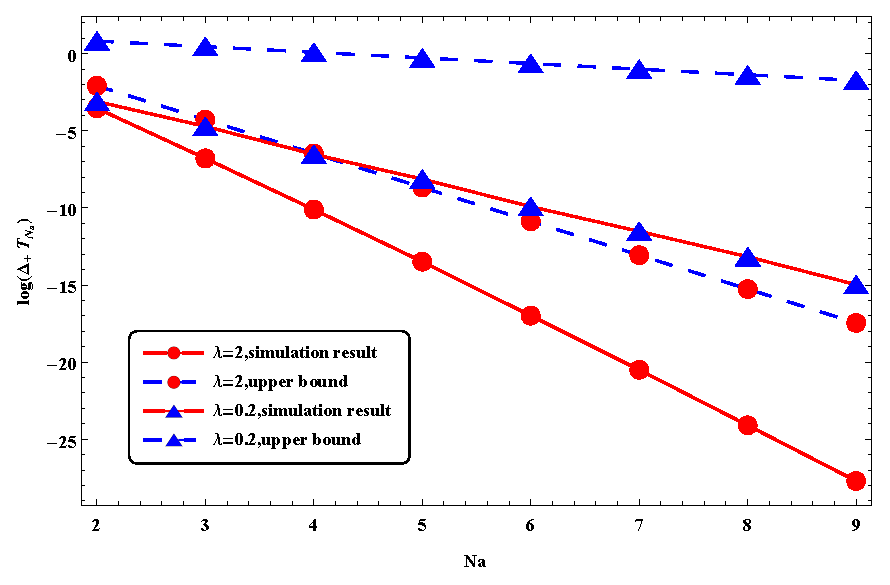
\includegraphics[width=280pt]{decreasing_exponential.eps}
%  \caption{连分式指数收敛性图示}\label{fig:continuous_fraction_exponential}
%\end{figure}
%\end{frame}
%\cfrac{1}{1+\cfrac{z^2}{3-z^2+\cfrac{(3z)^2}{5-3z^2-\cfrac{(5z)^2}{7-5z^2+ \cfrac{(7z)^2}{9-7z^2-\dots}}}}}
%\begin{frame}
%\begin{align*}
%\bm{K}_1&=\lambda \bm{I}_2+(1-\bm{u}_1^{\textrm{T}}\bm{K}_2^{-1}\bm{u}_1)\bm{u}_1\bm{u}_1^{\textrm{T}}\\
%\bm{K}_2&=\lambda \bm{I}_2+\bm{u}_1\bm{u}_1^{\textrm{T}}+(1-\bm{u}_2^{\textrm{T}}\bm{K}_3^{-1}\bm{u}_2)\bm{u}_2\bm{u}_2^{\textrm{T}}\\
%\dots & =\dots\\
%\bm{K}_n&=\lambda \bm{I}+\bm{u}_{n-1}\bm{u}_{n-1}
%\end{align*}
%$\bm{K}_1$的两个特征值是什么?
%
%一个特征值是$\lambda$,
%另一个特征值是$\tilde{\lambda}_1$
%设$\bm{u}_i$和$\bm{u}_{i+1}$的夹角是$\theta_i$,$\tilde{\lambda}_i$是$\bm{K}_i-\bm{u}_{i-1}\bm{u}_{i-1}^{\textrm{T}}$的不等于$\lambda$的那个特征值,$\bm{u}_{0}=\bm{0}$。
%\[
%\tilde{\lambda}_1=\lambda+\frac{1}{1+\frac{\sin^2\theta_1}{\lambda}+\frac{\cos^2\theta_1}{\tilde{\lambda}_2}}
%\]

%\[
%\arctan z
%=\cfrac{1}{1+\cfrac{z^2}{3-z^2+\cfrac{(3z)^2}{5-3z^2+\cfrac{(5z)^2}{7-5z^2+ \cfrac{(7z)^2}{9-7z^2-\dots}}}}},|z|<1
%\]
%上式令$z=1$得到无理数$\pi$的一种连分式展开
%\end{frame}
%\begin{frame}
%\[
%\sum_{x_1=1}^5\sum_{x_2=x_1}^5\dots\sum_{x_{12}=x_{11}}^5 1
%\]
%0<=x1<=x2<=...<=x12<=5,设r1=x1,r2=x2-x1,...r12=x12-x11,r13=5-x12,则
%\[
%r1+r2+\dots+r13=5,0\leq ri
%\]
%推出
%\[
%(r1+1)+(r2+1)+\dots+(r13+1)=17=1+1+\dots+1,1\leq ri+1
%\]
%从等式右边16个加号里取12个加号...
%\end{frame}
%
